\chapter{Grundlagen}
\label{cha:Grundlagen}

\section{Spill and Fill}
\section{Verwendung eines Spill and Fill Mechanismus in anderen Prozessoren}
\subsection{Sun Sparc Prozessoren}
Die Sun Sparc Prozessoren V8/V9 verf\"ugen \"uber ein sliding register Window mit jeweils 16 8 byte Registern in 7 Registers\"atzen. Sliding Window bezeichnet ein Verfahren, bei dem die Registers\"atze im Falle eines Funktionsaufruf nicht auf dem Stack gesichert werden m\"ussen, stattdessen wird auf den n\"achsten Registersatz gewechselt. Dabei wird meistens auch die Parameter\"ubergabe realisiert. Dabei sind die Input Register in dem Registerwindow des Callers identisch mit dem Output Registern, in dem Registerwindow des Callee.   
Mit speziellen Bytecode Instruktionen werden im Spill an Fill Verfahren Registers\"atze ausgetauscht, sobald diese nicht mehr ausreichen, was allerdings wegen den großen Registers\"atzen recht viel Zeit in Anspruch nimmt.
\section{AMIDAR}
Bei der Klasse der AMIDAR Prozessoren handelt es sich um ein konfigurierbares System bestehend aus Function Units (FU) f"ur die jeweiligen Aufgaben. Die FUs sind dabei untereinander mit einen Token- und einem Datennetzwerk verbunden. 
\subsection{Funktion}



\subsection{Framestack}

Die Framestack FU dient dazu die Funktionen des Operand Stacks und des Speichers f"ur lokale Variablen zur Verf"ugung zu stellen. 
Der AMIDAR Framestack arbeitet bei der Stackframe Verarbeitung mit drei grunds"atzlichen Zeigern. Der Stackpointer gibt die n"achste freie Speicheradresse "uber den aktuellen Stackframe an. Der Locals Pointer gibt die unterste Lokale Variable und damit auch das untere Ende des Stackframes an. Die dritte wichtige Zeiger ist der Callercontext Pointer, der auf die unterste Adresse des Callcontext deutet. 

\subsubsection{Stackframe}
Ein Stackframe beginnt mit den Parametern und den Lokalen Variablen.  Dar"uber kommt der Callercontext mit den alten Localspointer, Stackpointer und Callercontextpointer. Das obere Ende des Stackframes besteht aus dem Callercontext. 

\subsubsection{Funktionsaufrufe}
\begin{figure}
	\centering
	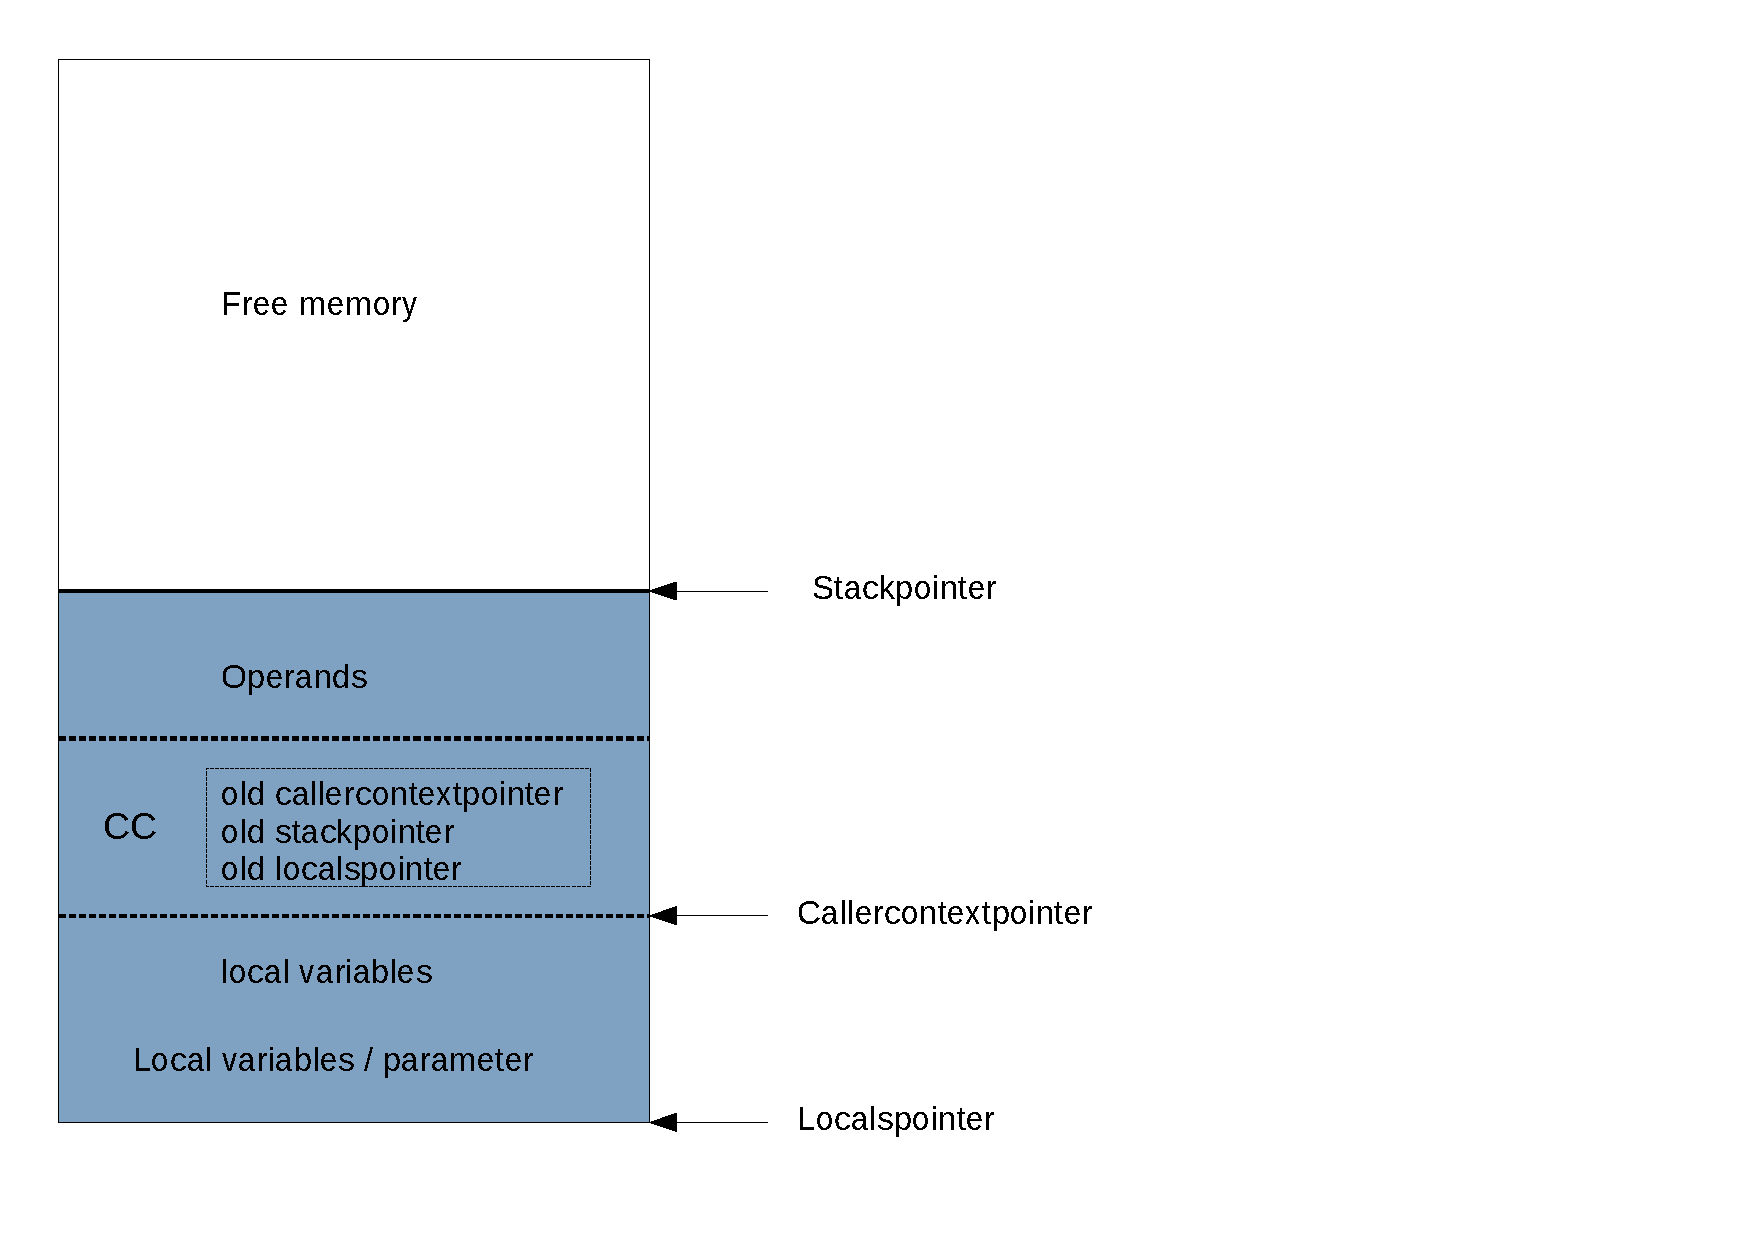
\includegraphics[height = 10cm]{PS_RS_graphics/Stackframe before Invoke.pdf}
	\caption{Stackframe vor einen Funktionsaufruf}
\end{figure}
Eine f"ur dieses Projekt wichtige Funktion des Framestacks sind Funktionsaufrufe. Bei einen Funktionsaufruf werden im Framestack die die 3 wichtigen Pointer neu gesetzt. Und der alte Callercontext gesichert. Der neue Localspointer wird berechnet in dem man vom aktuellen Stackpointer die Anzahl der Parameter der aufgerufenen Methode abzieht. Der neue Callercontextpointer wird berechnet indem auf dem neuen Localspointer die mit den Token "ubergebene Anzahl lokaler Parameter drauf addiert wird. Der neue Stackpointer wird berechnet, in dem auf dem Callercontextpointer die gr"o{ss}e des Callercontext drauf addiert wird. 
In den n"achten Takten werden die alten Localspointer, Stackpointer und in den Callercontextpointer geschrieben. 
\begin{figure}
	\centering
	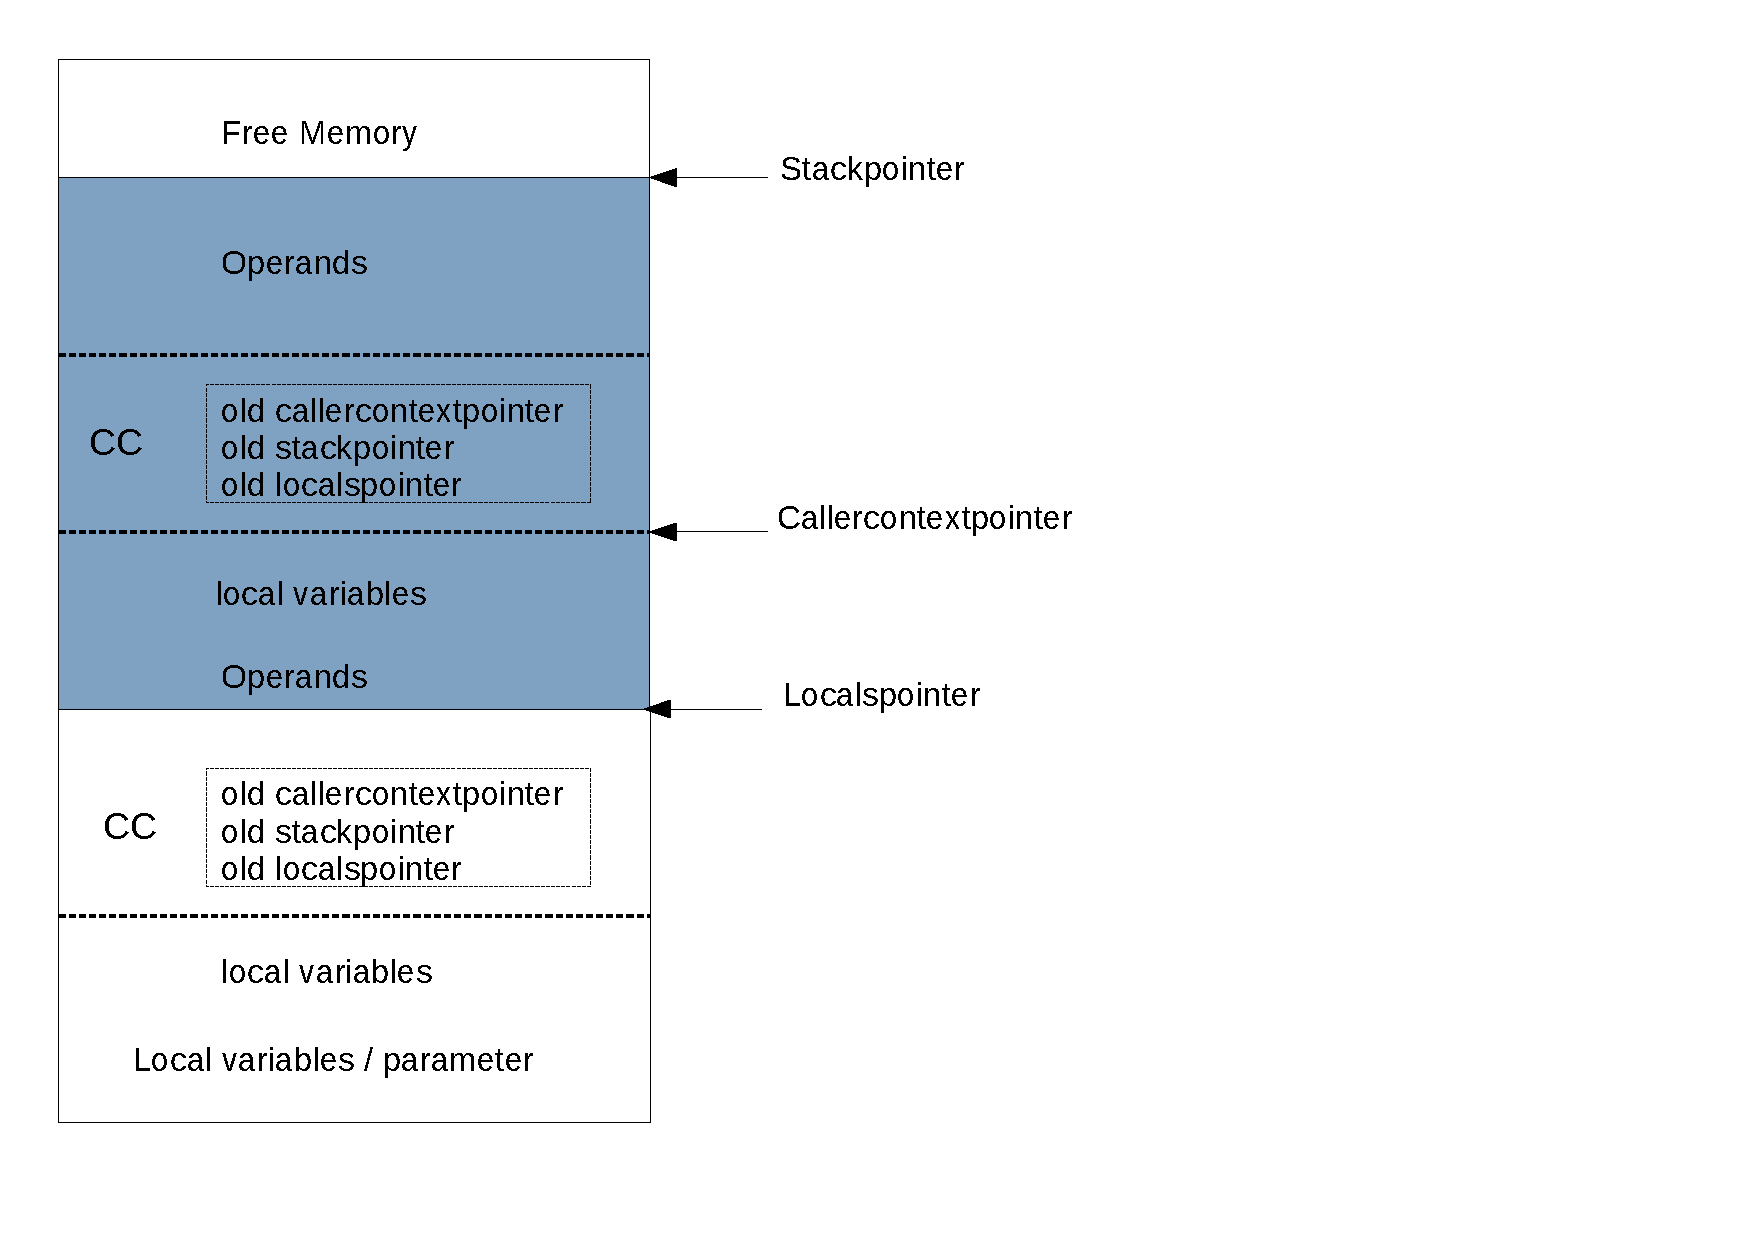
\includegraphics[height = 10cm]{PS_RS_graphics/Stackframe after Invoke.pdf}
	\caption{Stackframe nach einen Funktionsaufruf}
\end{figure}


\subsubsection{Funktionsr"ucksprung}

Bei einen Funktionsr"ucksprung werden im AMIDAR Framestack die Locals- Stack- und Callercontextpointer aktualisiert. Der Vorgang beginnt wenn eines der entsprechenden Token "uber den AMDIAR Bus gesendet wird. Es gibt 3 Varianten des Tokens. Einer liefert keinen R"uckgabewert, die anderen geben jeweils 32 oder 64 Bit zur"uck. Wenn der Token abgearbeitet wird, werden nacheinander die drei Pointer ausgelesen und wiederhergestellt. Anschlie{ss}end wird gegebenenfalls der R"uckgabewerte gesichert dieser steht in den "top of Stack" bzw. "next of stack" Registern. Der R"uckgabewert wird an stelle des obersten, im Falle eines Return64 der oberen beiden, Operanden des Urspr"unglichen Funktionsaufruf gespeichert. 

\begin{figure}
	\centering
	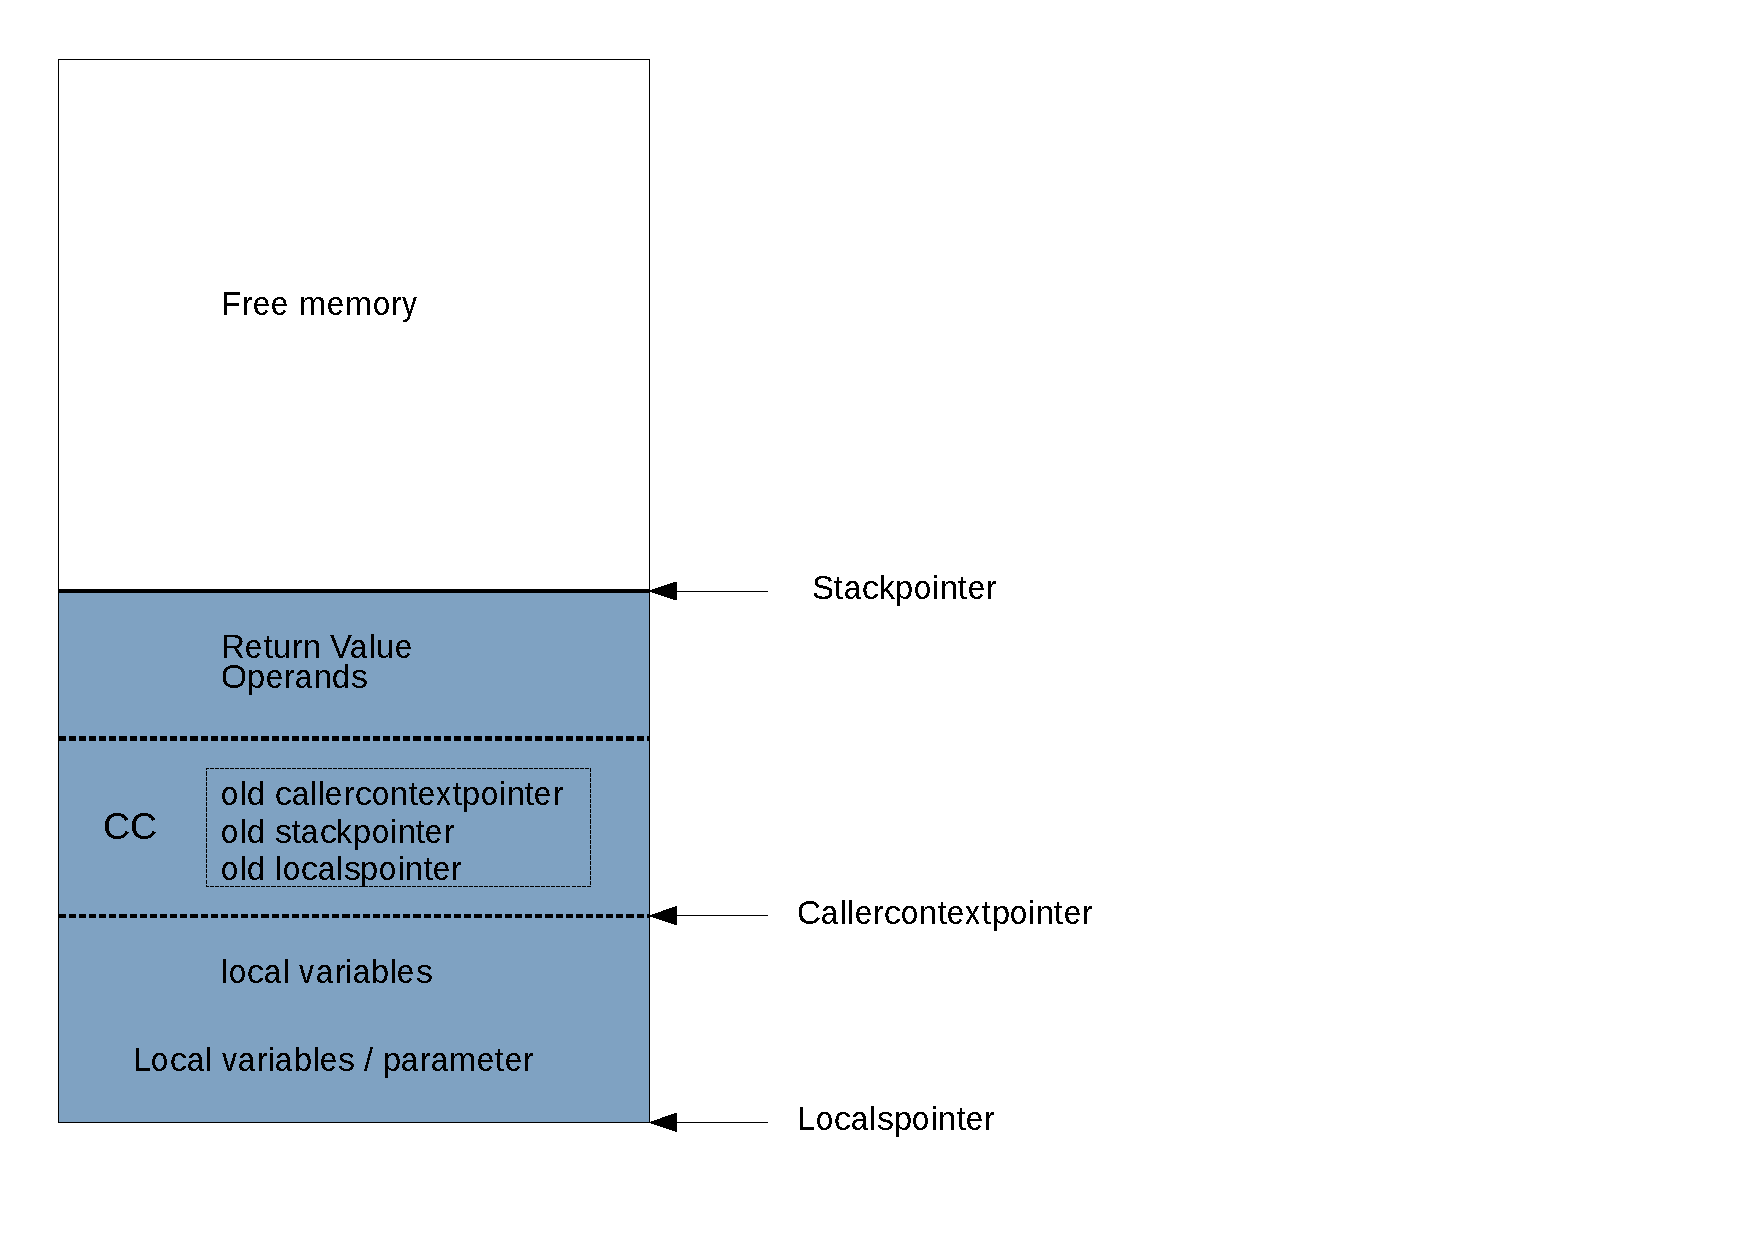
\includegraphics[height = 15cm]{PS_RS_graphics/Stackframe after return.pdf}
	\caption{Stackframe nach einen Funktionsr"ucksprung}
\end{figure}